%\documentclass{winnower}
\documentclass{article}
\usepackage{graphicx}
\usepackage[margin=0.9in]{geometry}
\begin{document}

\title{A Comparative Study of Generative Adversarial Networks}

\author{Cameron Fabbri}
%\affil{Computer Science and Engineering, University of Minnesota}
\date{4/24/2017}

\maketitle

\begin{abstract}
We provide an overview of Generative Adversarial Networks as a class of generative models for
image generation, and discuss how they can be applied towards the task of automatic image colorization. 
We first give a brief overview of Deep Learning and the recent advances in generative models.
We then discuss several varients of Generative Adversarial Networks, the problems they pose during training,
and theoretical methods towards stabalizing training.
\end{abstract}


%-------------------------------------------------%
\section{Introduction}
%-------------------------------------------------%
Deep learning has recently shown impressive results towards various problems in multiple domains such as speech recognition,
image classification, image segmentation, and reinforcement learning []. Until recently, much of the focus was towards
discriminative models, which aims to map a high-dimensional input, such as an image, to a class label. Deep generative models,
such as Deep Botlzmann Machines and Deep Belief Networks, have not had the same level of success.
Generative Adversarial Networks (GANs)[1] are a class of generative models that have shown great success in generatig realistic
images. Despite their success, they are known to be very difficult to train, and are extremely sensitive to modifications.
For this reason it is not yet straightforward to directly apply them towards a different problem.\newline

\noindent Since their introduction in 2014, there have been several large contributions made towards stabalizing and understanding
the training process of GANs. We discuss and compare four different objective functions used for training GANs:

\begin{itemize}
   \item Classification loss
   \item Least Squares loss
   \item Energy loss
   \item Wasserstein
\end{itemize}

\noindent We provide a background on deep learning in Section 2, and in Section 3 discuss the varients of GANs mentioned above.
Section 4 demonstrates these varients on the task of automatically colorizing grayscale images. The Appendix provides further
results from our experiments.

%-------------------------------------------------%
\section{Background and Related Work}
%-------------------------------------------------%

%-------------------------------------------------%
\subsection{Deep Learning}
%-------------------------------------------------%
Deep learning is a class of machine learning algorithms that use one or more \textit{hidden layers} between the input and output
to learn a heirarchy of concepts, often referred to as \textit{deep neural networks} (DNN).
In a feedforward network, or multilayer perceptron (MLP), each successive layer uses the output
from the previous layer as input, and uses an activation function, such as a logistic function, to obtain a new representation of the input. To
learn the set of weights and biases connecting successive layers, the error is propagated backwards through the network in order to optimize a
given objective function. This process is known as \textit{backpropogation}. Backpropogation is used in conjunction with an optimization method,
such as gradient descent, to effeciently compute the gradients by propogation from the output to input. This allows multi-layer networks to learn
a non-linear mapping from copious amounts of data. Because of the large amount of data needed to effectively train DNNs, \textit{stochastic gradient descent}
is often used via batches of data, which amounts to computing the gradient on a mini-batch of training samples. Recent advances in GPUs have
provided massive speedups in training due to their ability to parallelize the many operations in a DNN. \newline

%-------------------------------------------------%
\subsection{Convolutional Neural Networks}
%-------------------------------------------------%
\noindent The most common type of DNN for visual data is the Convolutional Neural Network (CNN), which is designed specifically for
multidimensional data such as images. CNNs incorporate three powerful techniques in order to achieve some degree of scale and shift invariance.
The first is the use of shared weights, which stems from the idea that a feature detector used in one part of an image is almost certainly useful in
other parts of the image. This also allows networks to reduce the number of parameters to avoid the curse of dimensionality. The second is the use of
local receptive fields. A kernel or filter is \textit{convolved} across the entire
image to produce a \textit{feature map}. Each pixel in the resulting feature map is the result of the kernel convolved with a small area in the input.
The use of local receptive fields allow earlier layers in the network to learn low-level features such as edges or corners, which can then be combined
in successive layers throughout the network to learn high-level features. The third technique is various forms of subsampling, such as the use of pooling
layers, which provide a form of nonlinear downsampling. Subsampling is performed to reduce the dimensionality of the internal representation. \newline

\noindent While the size of the output in a MLP is independent of the size of its input,
the height and width of the resulting feature maps are dependent on the size and stride of the kernel. The number of feature maps or \textit{depth} of the
resulting layer (which corresponds to the \textit{width} of the network as a whole) however, is arbitrary. Clearly, there are many different opitions to be chosen,
such as the size of the kernel, the stride of the kernel, depth of the . When designing a CNN, many rely on heuristics, as well as theorectical
design principles as shown in [inception paper]. An example CNN architecture is shown in Figure 1. \newline

%-------------------------------------------------%
\subsection{Deep Generative Models}
%-------------------------------------------------%
\noindent Much focus has been put on CNNs as a discriminative model, learning a function to map some input data to some desired output label. In other words,
they learn the conditional distribution $P(y|x)$. The rest of this paper is focused on \textit{generative} models, which instead learn the joint
probability of the input data and labels. They attempt to model the data directly by learning $P(x,y)$. Autoencoders, Deep Boltzmann Machines, and
Deep Belief Nets are some examples of these class of models.

\begin{figure}[!htb]
   \begin{center}$
      \begin{array}{cccc}
         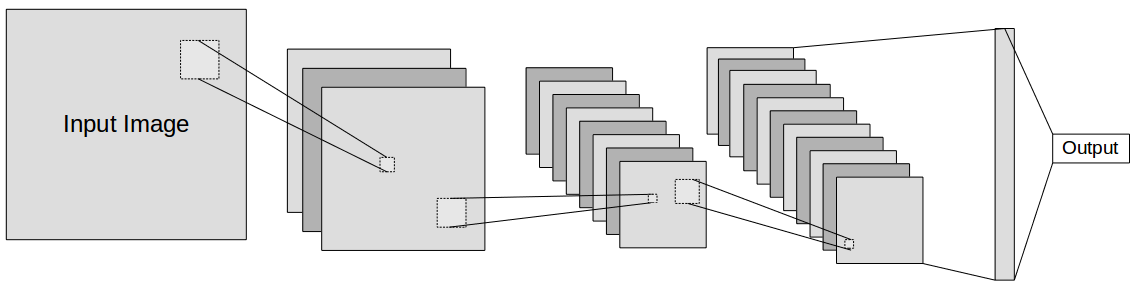
\includegraphics[width=5in]{cnn}
      \end{array}$
   \end{center}
   \caption{An example of a Convolutional Neural Network}
\end{figure}

%-------------------------------------------------%
\section{Generative Adversarial Networks}
%-------------------------------------------------%
\noindent Generative Adversarial Networks (GANs) 

%-------------------------------------------------%
\subsection{Conditional Generative Adversarial Networks}
%-------------------------------------------------%

%-------------------------------------------------%
\subsection{Deep Convolutional GANs}
%-------------------------------------------------%

%-------------------------------------------------%
\subsection{Least Squares GANs}
%-------------------------------------------------%


%-------------------------------------------------%
\subsection{Energy-Based GANs}
%-------------------------------------------------%	 


%-------------------------------------------------%
\subsection{Wasserstein GANs}
%-------------------------------------------------%


%-------------------------------------------------%
\section{Colorization}
%-------------------------------------------------%
We now show how adversarial networks can be used for generating a plausible color version of a grayscale image.
The problem is set up as a cGAN, where the generator and descriminator are both conditioned on the grayscale image.






\bibliographystyle{abbrvnat}
[1] Graves, Alex, and Navdeep Jaitly. "Towards End-To-End Speech Recognition with Recurrent Neural Networks." ICML. Vol. 14. 2014.
[2] Goodfellow, Ian, Yoshua Bengio, and Aaron Courville. Deep learning. MIT Press, 2016.
\bibliography{winnower_template}

\appendix

\section{Appendix}
Here we show 


\end{document}
